China's official external lending is predominantly undertaken by state-owned entities and the government itself\footnotemark{}. However, unlike other major economies, the Chinese government does not report or publish any data on its official international lending or outstanding overseas debt claims. This lack of transparency creates challenges for rating agencies, as official lending to sovereigns is not a regular part of their activities. Moreover, China is not a member of the Paris Club, which tracks sovereign borrowing from official bilateral creditors, and does not divulge data on its official flows with the OECD's Creditor Reporting System \citep*{Horn-Reinhart-Trebesch-21}.
\footnotetext{These include China's state-owned policy banks, such as China Development Bank (國家開發銀行, CDB) and China Export-Import Bank (中國進出口銀行, Ex-Im), as well as China's state-owned commercial banks such as Industrial and Commercial Bank of China (中國工商銀行, ICBC) or Bank of China (中國銀行, BoC)}

\citet*{Horn-Reinhart-Trebesch-21} combines a variety of sources to construct a consensus database of Chinese official loans.
The HRT database spans from 1949, the establishment of the People's Republic of China, to 2017. It contains a granular dataset of 2151 loans and 2824 grants with information such as the creditor agent, borrower type, commitment, maturity, etc. It also provides an aggregate panel data of the external debt to China for each country.
\begin{figure}[t]
    \centering
    \begin{subfigure}[t]{0.45\textwidth}
        \centering
        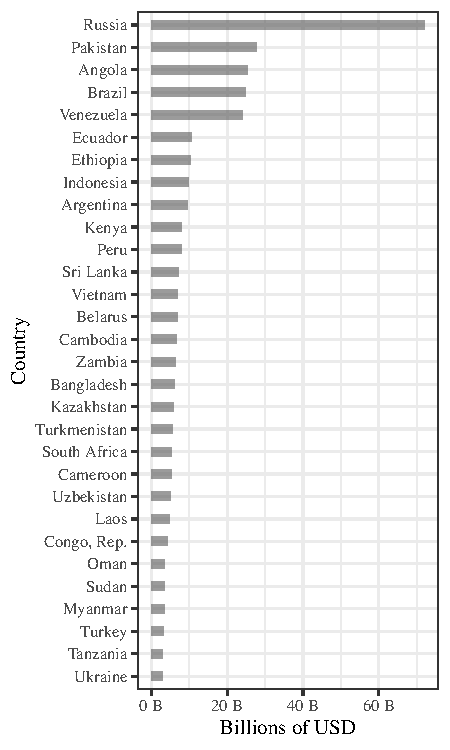
\includegraphics[width = \textwidth]{fig/total_debt.pdf}
        \caption{Top 30 Debtor by Total Debt in USD}
        \label{fig:total-debt-30}
    \end{subfigure}%
    ~
    \begin{subfigure}[t]{0.45\textwidth}
        \centering
        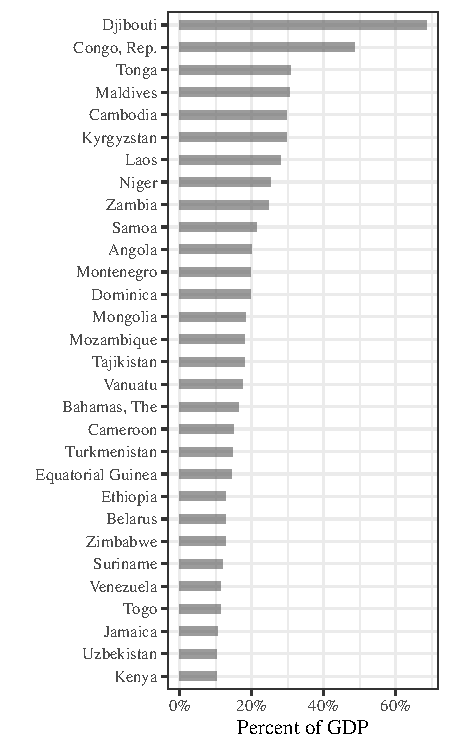
\includegraphics[width = \textwidth]{fig/perc_debt.pdf}
        \caption{Top 30 Debtor by Dept-to-GDP Ratio}
        \label{fig:perc-debt-30}
    \end{subfigure}
    \caption{Debt to China Statistic by Country in 2017}
    \label{fig:Country-Agg}
    \floatfoot{Source: HRT Database \citeyearpar{Horn-Reinhart-Trebesch-21} \\
    Note: The figure on the left presents the top 30 countries in amount of total external debt to China in 2017. The figure on the right compares by the China-debt-to-GDP ratio.}
\end{figure}

The top 30 countries with the largest debts to China's official creditors are displayed in \autoref{fig:total-debt-30}. Notably, Russia owes China over \$70 billion, while Pakistan's debt amounts to \$27 billion, both topping the list. Brazil and Venezuela are among the top 10 countries with the highest debt to China in Latin America. Contrary to what many people believe, African countries have not borrowed much from China. However, if we consider the ratio of Chinese debt to GDP in \autoref{fig:perc-debt-30}, some African countries appear to be highly indebted to China. Djibouti, for instance, has an alarming ratio of 68.5\% of its GDP consisting of Chinese debt, while Tonga, Niger, and Zambia have ratios exceeding 10\%.
\begin{figure}
    \centering
    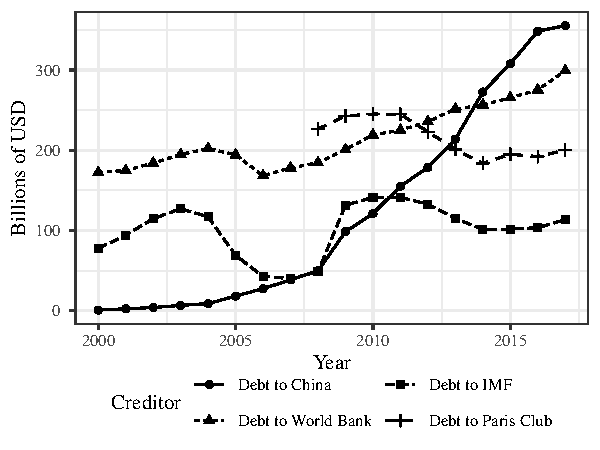
\includegraphics[width = 0.7\textwidth]{fig/aggr_debt_source.pdf}
    \caption{Change of Aggregate Public Debt for Different Official Creditors}
    \label{fig:debt-ts}
    \floatfoot{Source: HRT Database \citeyearpar{Horn-Reinhart-Trebesch-21} \\
    Note: The figure shows the change in the aggregate external public debt that the developing countries owed to different official creditors. These include China, World Bank (excluding China), IMF, and all 22 Paris Club governments. It is obvious that China had become the largest official creditors in the world according to the estimation of \citet*{Horn-Reinhart-Trebesch-21}.}
\end{figure}

A main finding in \citet*{Horn-Reinhart-Trebesch-21} is that China had become the world's largest creditor to developing countries after 2013, surpassing the amount of World Bank. \autoref{fig:debt-ts} shows the change of the total amount of debt from different main creditors, including China, World Bank\footnote{Including the International Development Association (IDA) and the International Bank for Reconstruction and Development (IBRD) }, IMF, and the aggregation of all countries in the Paris Club. The debt amount started to rise rapidly after 2000, when the China government launched the ``Go Out Policy'' in 1999. In 2017, the debt to China had reached \$355 billion, while the debt to World Bank was \$300 billion.


This database allows researchers to obtain the true amount of total debt of a country, and gauge the amount of debt that is considered superfluous and onerous for it.
For the next section, I briefly explain the two countries I will examine in my thesis, and demonstrate the importance of choosing it as a benchmark example.